\documentclass[12pt]{book}

\newcommand{\bhtAuthor}{Wilfried Pahl}
\newcommand{\bhtTitle}{Klassifizierung für E-Commerce Nutzergruppen auf Basis von Data Mining unter Verwendung von künstlicher Intelligenz.}
\newcommand{\bhtSubtitle}{Untersuchung der Nutzerklassifizierung durch Datenanalyse}
\newcommand{\bhtDocumentType}{Masterarbeit}
\newcommand{\bhtDegree}{Master of Science (M.Sc.)}
\newcommand{\bhtMatriculationNumber}{901932}
\newcommand{\bhtCourse}{Online Medieninformatik}
\newcommand{\bhtTown}{Temmen-Ringenwalde}
\newcommand{\bhtUniversity}{Berliner Hochschule für Technik}

\newcommand{\bhtContributorFirst}{Prof. Dr. S. Edlich ~Berliner Hochschule für Technik}
\newcommand{\bhtContributorSecound}{noch nicht bekannt ~auch von einer Hochschule}

\usepackage[a4paper,width=150mm,top=25mm,bottom=25mm]{geometry}

\usepackage[OT1]{fontenc}
\renewcommand*\familydefault{\sfdefault}

\usepackage[utf8]{inputenc}
\usepackage[ngerman]{babel}

\usepackage{graphicx}
\graphicspath{
	{images/}
}

\usepackage[dvipsnames]{xcolor}

\usepackage{fancyhdr}

\fancyhead{}
%\fancyhead[RO,LE]{\bhtTitle}
\fancyfoot{}
%\fancyfoot[LE,RO]{\thepage}
%\fancyfoot[CO,RE]{\bhtAuthor}
\renewcommand{\headrulewidth}{0.4pt}
\renewcommand{\footrulewidth}{0.4pt}


%%%%%%%%%%%%%%%%%%%%%%%%%%%%%%
% interne/externe Links
%%%%%%%%%%%%%%%%%%%%%%%%%%%%%%
\usepackage[
colorlinks,
pdfpagelabels,
pdfstartview=FitH,
bookmarksopen=true,
bookmarksnumbered=true,
plainpages=false,
hypertexnames=false,
backref=true,
pagebackref=true,
hyperindex=true,
breaklinks=true,
linkcolor=darkgray,
citecolor=darkgray,
urlcolor=darkgray
]{hyperref}

% Text durchgestrichen: \sout{Test}
\usepackage[normalem]{ulem}

\parindent0cm

\usepackage{draftwatermark}
\SetWatermarkText{\textbf{ENTWURF}}
\SetWatermarkScale{4}


\usepackage{glossaries}
\newglossaryentry{stakeholder}
{
name=Stakeholder,
description={Stakeholder oder Projektbeteiligte sind alle Personen, Institutionen und Dokumente, die von der Entwicklung und vom Betrieb eines Systems in irgendeiner Weise betroffen sind. Dazu gehören auch Personen, die nicht in der Systementwicklung mitwirken, aber das neue System zum Beispiel nutzen, in Betrieb halten oder schulen}
}
\newglossaryentry{verantwortungsdiffusion}
{
	name=Verantwortungsdiffusion,
	description={bezeichnet das Phänomen, dass eine Aufgabe, die offensichtlich zu tun ist, nicht ausgeführt wird – obwohl dafür genügend fähige Personen anwesend beziehungsweise verfügbar wären}
}
\newglossaryentry{planning_poker}
{
	name=Planning Poker,
	description={als eine Variante der Aufwandsschätzung ist in den Scrum-Kreis\-lauf eingebettet. Dabei kommt es in den Sprint Planning Meetings zur Anwendung, meist wenn ein neues Product Backlog geschrieben worden ist. Beim Planning Poker ist man darauf bedacht, spielerisch die Erreichung von Konsens innerhalb eines Teams zu erwirken}
}
\newglossaryentry{storyboards}
{
	name=Storyboards,
	description={ähneln Szenarien mit denen Interaktion veranschaulichen werden, die erforderlich sind, um ein Ziel zu erreichen. Anstatt eine Liste von Schritten dazustellen, visualisiert ein Storyboard die Interaktion ähnlich wie ein Comic}
}
\newglossaryentry{personas}
{
name=Personas,
description={stellt einen Prototyp für eine Gruppe von Nutzern dar, mit konkret ausgeprägten Eigenschaften und einem konkreten Nutzungsverhalten}
}
\newglossaryentry{personas_driven_user_stories}
{
	name=Personas-driven User Stories,
	description={sind User Stories die eine konkrete Persona verwenden und die User Storie wird für eine bestimmte Personengruppe, die im Persona definiert wurde, erstellt. Es wird also nicht \glqq Als Anwender möchte ich ...'', verwendet, sondern beispielsweise \glqq Als Peter möchte ich ...''}
}
\newglossaryentry{low_fi_prototypen}
{
	name=Low-Fi Prototypen,
	description={ist ein Prototyp bei dem der Fokus auf Benutzerführung und Funktionalität weitestgehend losgelöst vom Design liegt.  Es ist eine (interaktive) Präsentation eines digitalen Produkts, wie beispielsweise einer Website oder einer App, die möglichst weit am Anfang des Entwicklungsprozesses steht, mit nur einigen viuellen Aspekten des Endproduktes}
}
\newglossaryentry{countinuous_integration}
{
	name=Countinuous Integration,
	description={ist ein Begriff aus der Software-Entwicklung, der den Prozess des fortlaufenden Zusammenfügens von Komponenten zu einer Anwendung beschreibt. Das Ziel der kontinuierlichen Integration ist die Steigerung der Softwarequalität}
}
\newglossaryentry{continuous_delivery}
{
	name=Continuous Delivery,
	description={bezeichnet eine Sammlung von Techniken, Prozessen und Werkzeugen, die den Software-Auslieferungsprozess verbessern. Die Automatisierung der Integrations- und Auslieferungsprozesse ermöglicht schnelle, zuverlässige und wiederholbare Deployments. Erweiterungen oder Fehlerkorrekturen können somit mit geringem Risiko und niedrigem manuellem Aufwand in die Produktivumgebung oder zum Kunden ausgeliefert werden}
}
\newglossaryentry{ux_schulden}
{
	name=UX-Schulden,
	description={bezeichnet die Kluft zwischen aktueller UX und der künftigen UX, die nach Begleichen der UX-Schulden vorhanden sein könnten}
}
\newglossaryentry{technischen_schulden}
{
	name=technischen Schulden,
	description={Technische Schulden oder Technische Schuld (englisch technical debt) ist eine in der Informatik gebräuchliche Metapher für die möglichen Konsequenzen schlechter technischer Umsetzung von Software. Unter der technischen Schuld versteht man den zusätzlichen Aufwand, den man für Änderungen und Erweiterungen an schlecht geschriebener Software im Vergleich zu gut geschriebener Software einplanen muss}
}
\newglossaryentry{hci}
{
	name=HCI,
	description={(\textit{englisch Human–computer interaction}) erforscht das Design und die Verwendung von Computer-Technologie an der Schnittstelle zwischen Menschen (Anwendern) und Computern. Forscher auf dem Gebiet der HCI beschäftigen sich mit der Art und Weise, wie Menschen mit Computern und Design-Technologien interagieren}
}
\newglossaryentry{heuristische_evaluation}
{
	name=Heuristische Evaluation,
	description={(Heuristik – zu griech. heuriskein ‚finden‘) ist eine Methode, um die Gebrauchstauglichkeit einer Benutzeroberfläche vor Fertigstellung des Gesamtsystems zu beurteilen}
}
\newglossaryentry{content_management_system}
{
	name=CMS,
	description={Nutzerfreudliche Bedienungsoberfläche einer Software.}
}

\makeglossaries

\usepackage{makeidx}
\makeindex

\begin{document}
	\frontmatter % only for documentclass book
	\begin{titlepage}
	\begin{center}
		\vspace*{1.5cm}
		{\Huge \textbf{\bhtTitle}}

		\vspace*{0.5cm}
		{\large \textbf{\bhtSubtitle}}

		\vspace*{1cm}
		{\includegraphics[width=0.7\linewidth]{logo-bht.png}}
	\end{center}

	\vspace*{2cm}
	
	\begin{tabular}{ll}
		\multicolumn{2}{l}{vorgelegte \bhtDocumentType}\\
		\multicolumn{2}{l}{zum Erlangen des akademischen Grades}\\
		\multicolumn{2}{l}{\textbf{\bhtDegree}}
	\end{tabular}

	\vspace*{0.5cm}

	\begin{tabular}{ll}
		eingereicht von: & \bhtAuthor\\
		& Matrikelnummer: \bhtMatriculationNumber\\
		& Studiengang: \bhtCourse\\
		& \bhtUniversity\\
		& \\
		\textbf{Betreuender Prüfer} & \bhtContributorFirst \\
		\textbf{Zweitgutachter} & \bhtContributorSecound
	\end{tabular}

	\vspace*{2cm}
	\bhtTown, der \today
\end{titlepage}

	{\Large \textbf{Stichworte}}\vspace{0.1cm}

Data-Mining, Big Data, künstliche Intelligenz, Clusterung, Nutzergruppen, k-Means-Algorithm.\vspace{0.5cm}

{\Large \textbf{Kurzzusammenfassung}}\vspace{0.1cm}

Hier kommt das Abstract auf Deutsch.

	\newpage

	{\Large \textbf{Keywords}}\vspace{0.1cm}

Data-Mining, Big Data, künstliche Intelligenz, Clusterung, Nutzergruppen, k-Means-Algorithm.\vspace{0.5cm}

{\Large \textbf{Abstract}}\vspace{0.1cm}

Here comes later the abstract on German.

	\newpage
	
	{\Large \textbf{Danksagung}}\vspace{0.1cm}

Hier sage ich auch mal zu irgendjemand Danke.
	\newpage
	
	{\Large \textbf{Eidesstattliche Erklärung}}\vspace{0.1cm}

Hiermit erkläre ich, dass ich die vorliegende Arbeit selbstständig verfasst habe, dass ich sie zuvor an keiner anderen Hochschule und in keinem anderen Studiengang als Prüfungsleistung eingereicht habe und dass ich keine anderen als die angegebenen Quellen und Hilfsmittel benutzt habe. Alle Stellen der Arbeit, die wörtlich oder sinngemäß aus Veröffentlichungen oder aus anderweitigen fremden Äußerungen entnommen wurden, sind als solche kenntlich gemacht.\vspace{2.0cm}

\hrule\vspace{0.2cm}

{\small{Datum}}\hfill{\small{Unterschrift}}

	\newpage

	\tableofcontents
\addcontentsline{toc}{chapter}{Inhaltsverzeichnis}

%\clearpage
\listoffigures
\addcontentsline{toc}{chapter}{Abbildungsverzeichnis}


%\clearpage
\listoftables
\addcontentsline{toc}{chapter}{Tabellenverzeichnis}

	
	\mainmatter  % only for documentclass book
	%\pagestyle{fancy}
	\chapter{Einführung}
Das Volumen der bestellten Waren im E-Commerce Bereich wächst stetig und durch die \Gls{corona}-Krise erfuhr dieser Prozess eine Beschleunigung. Die meisten Umsätze verzeichnen virtuelle Marktplätze, wie Amazon und Ebay, aber auch kleine Onlineshops können durchaus bestehen.

\begin{figure}[!ht]
	\centering
	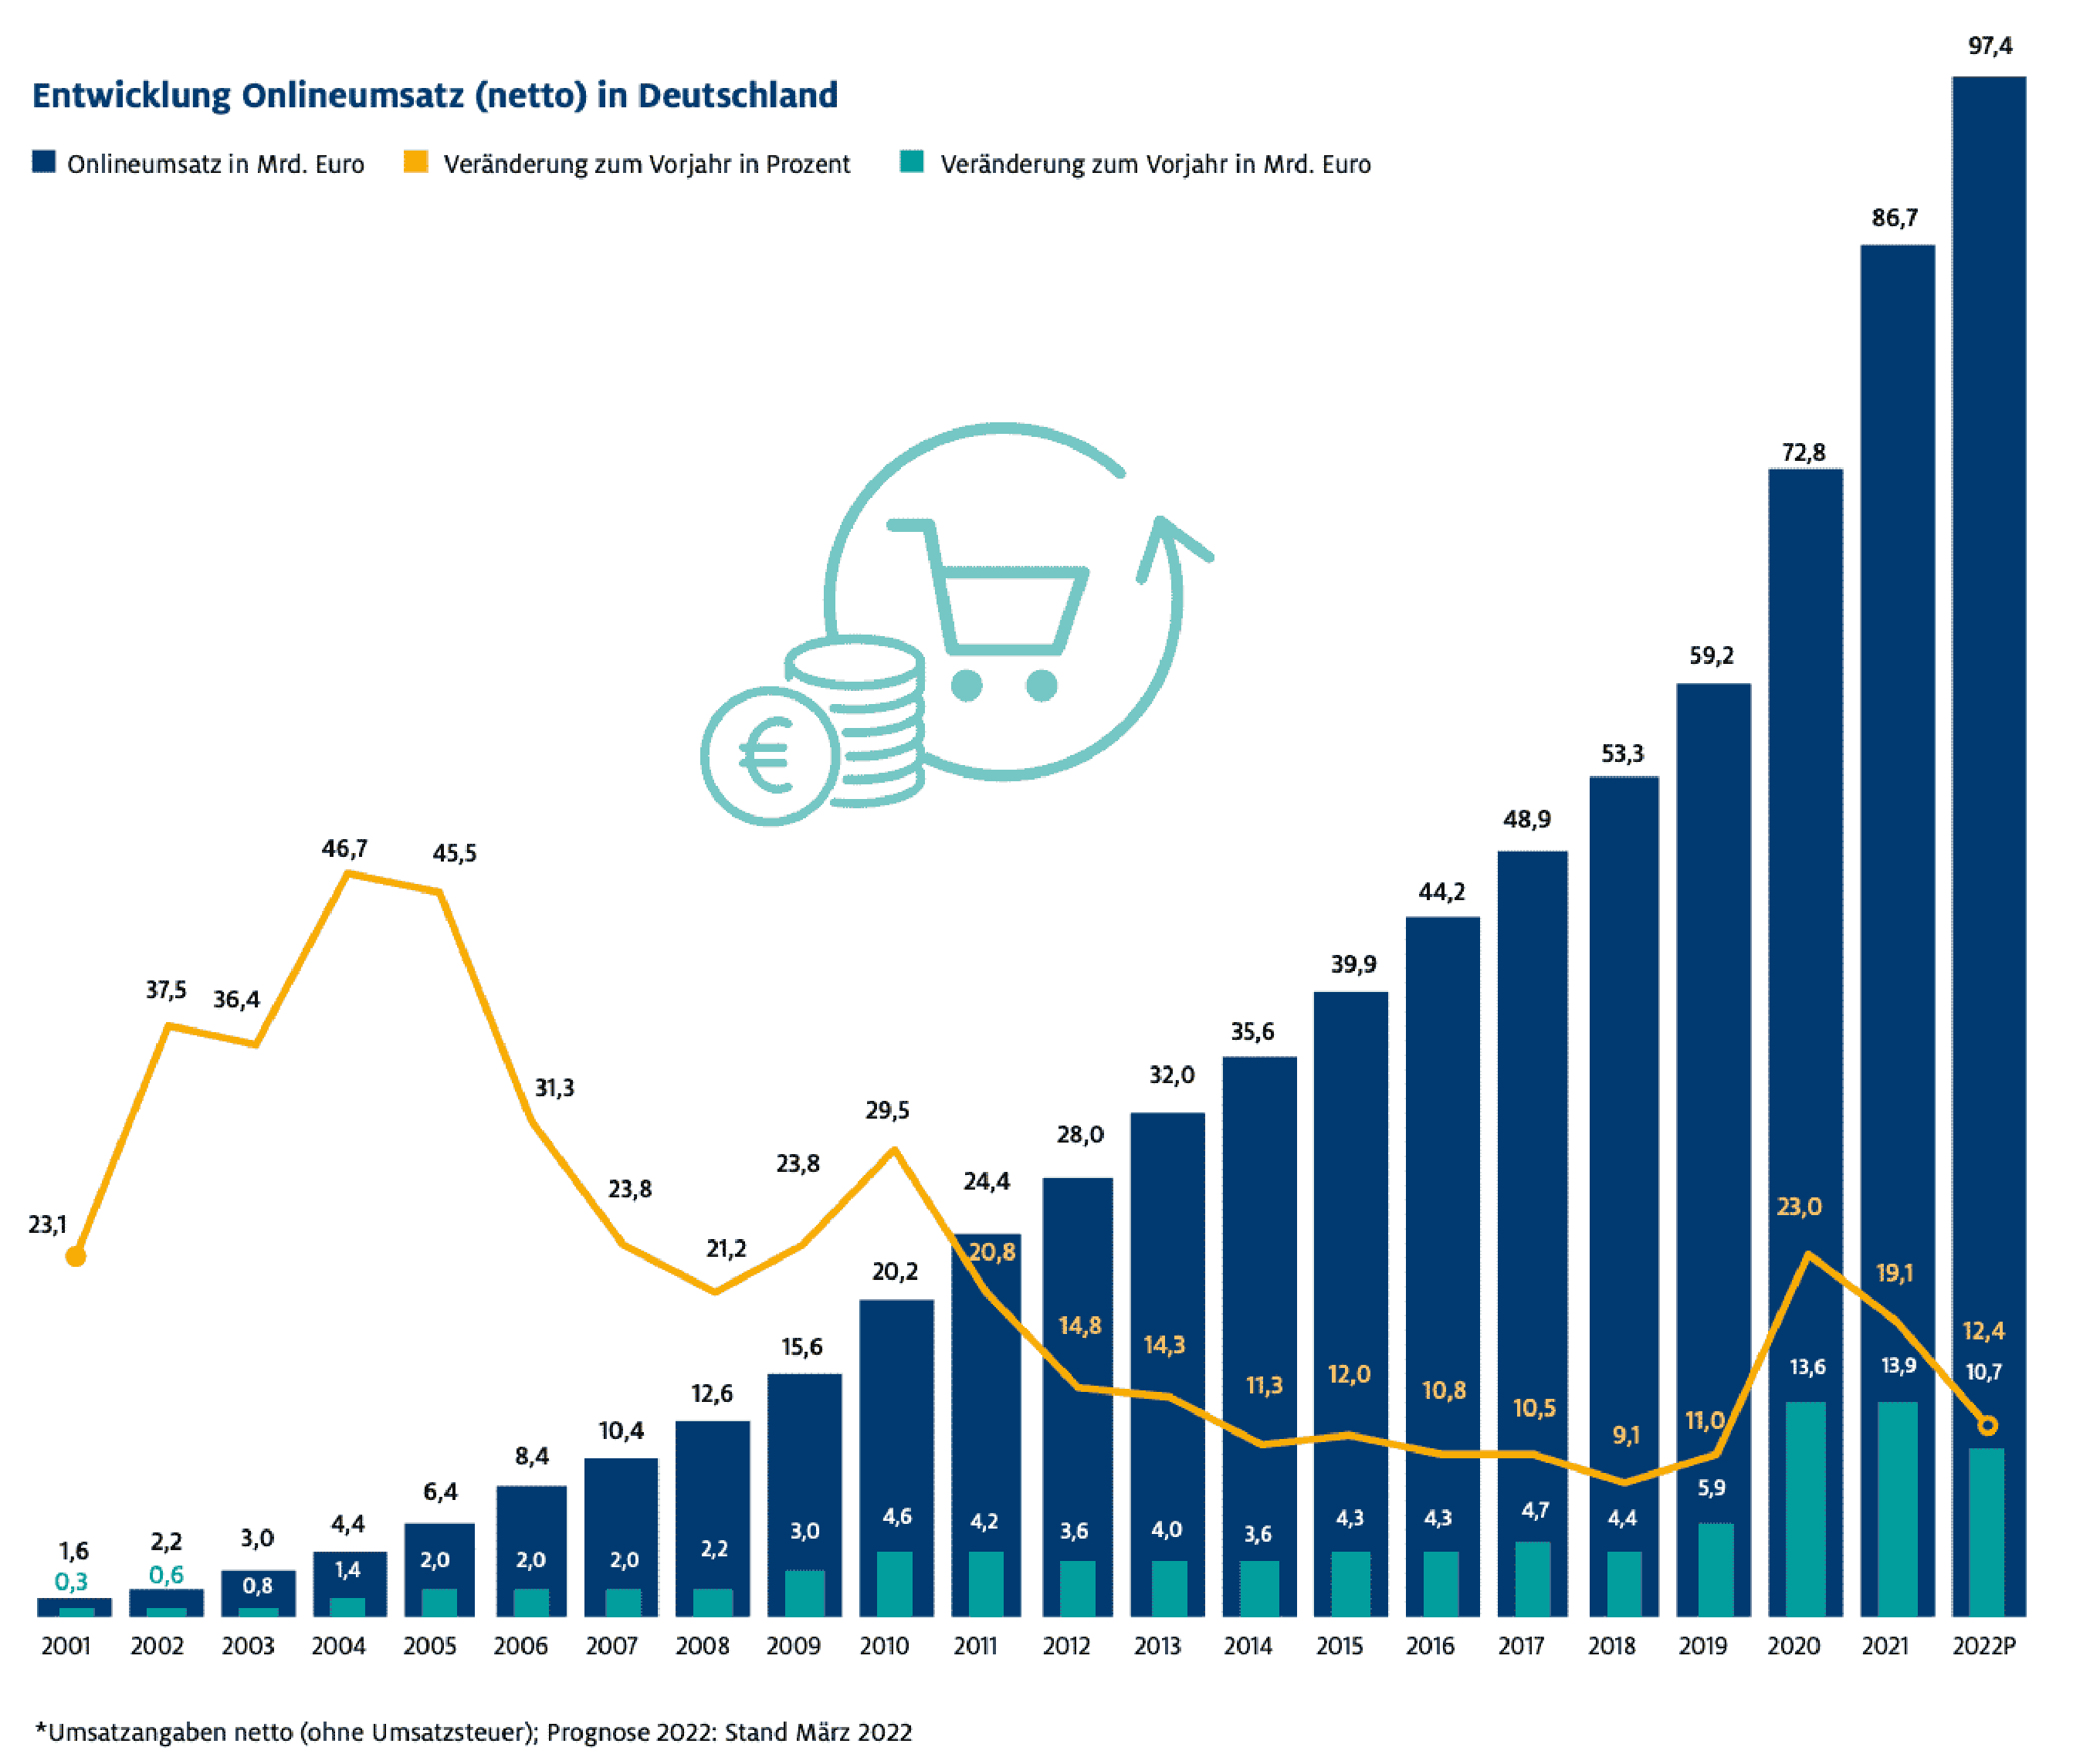
\includegraphics[width=\linewidth]{images/chapter1/umsatzprognose_2022.eps}
	\caption{Umsatzentwicklung E-Commerce von 2001-2022 \cite{ecommerce_statistics:versteegen2022}}
	\label{img:stat_prognose_2022}
\end{figure}

Mithilfe von Machine Learning können aus vorhandenen Daten, Nutzergruppe bestimmt werden, mit deren Hilfe besser Angebote für die Nutzergruppen erstellt und ausgespielt werden können.
\section{Motivation}
Im E-Commerce nutzen Onlineshop Betreiber Kundenklassifizierungen, um Kunden einzuteilen und ihnen besser Angebote unterbreiten zu können. Oft sind diese Klassifizierungen in den ersten Schritten bei der Shop-Planung oder bei einem \Gls{relaunch} erstellt wurden, basierend auf einer erwarteten und anvisierten Kundengruppe. In vielen Fällen werden keine Kundenklassifizierungen erstellt. Es wird unterstellt das alle Menschen zur Zielgruppe gehören.
\subsection{Ausgangslage}
Im Rahmen dieser Arbeit soll ein kleiner Onlineshop eines Verlages aus dem Nordosten Deutschlands untersucht werden. Über den Shop werden hauptsächlich Print-Produkte wie Bücher und Zeitschriften. Eine vorherige Planung und Analyse der Nutzergruppen und ihrer Bedürfnisse sind einigen Mitarbeitern, die den Shop betreuen, nicht wichtig.\vspace{0.2cm}

Folgende Aussagen trafen Mitarbeitern, die unmittelbar mit den Onlineshop Arbeiten und diesen betreuen.„Für den Onlineshop benötigen wir keine Nutzergruppen, dafür haben wir die verschiedene Menüpunkte. Nutzergruppen werden erst interessant, wenn wir auf verschiedenen Kanäle Werbung schalten.“ Aussage einer Mitarbeiterin für Kundenmanagement. „Zielgruppendefinition ist wichtig, aber für den Shop sollte keine angefertigt werden.“ Aussage einer Mitarbeiterin des Webdesigner Teams.
\subsection{Vorteile durch die Vorhersage}
Einer der wichtigsten Vorteile einer durch künstlicher Intelligenz vorhergesagten Nutzergruppenklassifizierung wäre das Ausschließen des menschlichen Einwirkens. Das Erhöht die Genauigkeit der Entscheidungen und es passieren weniger Fehler. Des Weiteren erkennt künstliche Intelligenz versteckte Muster aus tausenden und mehr Datensätzen. Ein weiterer Vorteil ist die Möglichkeit einer zeitnahen Anpassung der Verkaufsprozesse auf der Webseite und eine kontinuierliche Optimierung des Onlineauftritts.
\section{Ziel der Arbeit}
In dieser Arbeit ist die Prüfung, ob eine mögliche Vorhersage der Nutzergruppenklassifizierung durch künstliche Intelligenz möglich ist und ob diese Vorhersage Vorteile gegenüber einer klassischen Klassifizierung, beispielsweise durch Personas ist. Für die Vorhersage werden vorhandene Daten aus dem Shop und verschiedene externe Quellen verwendet.\vspace{0.2cm}

Durch die Zielsetzung lässt sich folgende Forschungsfrage und dazugehörige Unterfragen formulieren:\vspace{0.2cm}

„Ist die Erstellung eine Nutzergruppenklassifizierung mit Machine-Learning besser als eine klassische Analyse der Nutzergruppen?“

\begin{itemize}
	\item Welche Systeme und Algorithmen eignen sich am besten für die Klassifizierung?
\end{itemize}
\section{Inhaltlicher Aufbau der Arbeit}
Diesen Teil schreibe ich während der Fertigstellung der einzelnen Kapitel.

\chapter{Grundlagen}
\section{Grundbegriffe}

\textbf{Big Data}\vspace{0.2cm}

Eine Abgrenzung des Begriff Big Data ist nicht eindeutig, da der Begriff sehr heterogen verwendet wird. Somit gibt es viele Definitionen vom Begriff Big Data.\vspace{0.2cm}

Als Big Data werden Daten bezeichnet, die entweder zu groß, zu komplex, zu schnelllebig oder zu schwach strukturiert sind, um diese mit herkömmlichen Methoden auszuwerten. Big bezieht sich in der Definition auf die vier Dimensionen. In Big Data sind Technologien die richtigen Informationen dem richtigen Adressaten zur richtigen Zeit in der richtigen Menge am richtigen Ort und in der erforderlichen Qualität bereitstellen.\vspace{0.2cm}

Auch strukturierte Daten. Verschiedene (autonome) Datenquellen (Datenbanken oder Anwendungen).\vspace{0.2cm}

Auf volume (Umfang, Datenvolumen), velocity (Geschwindigkeit, mit der die Datenmengen generiert und transferiert werden), variety (Bandbreite der Datentypen und -quellen) und veracity (Echtheit von Daten).\vspace{0.5cm}

\textbf{Knowledge Discovery in Data (-base)}\vspace{0.2cm}

Dies hat das Ziel aus vorhandenen meist großen Datenbeständen, fachliche Zusammenhänge zu erkennen. Zu den Teilschritten des KDD Prozesses gehören 1. Bereitstellung von Hintergrundwissen, 2. Definition der Ziele, 3. Datenauswahl, 4. Datenbereinigung, 5. Datenreduktion, 6 Auswahl eines Modells, 7. Data-Mining, die eigentliche Datenanalyse, 8. Interpretation der gewonnenen Erkenntnisse.\vspace{0.5cm}

\textbf{Data-Mining}\vspace{0.2cm}

Data-Mining die systematische Anwendung von statischen Methoden auf große Datenbestände, um neue Querverbindungen zu erkennen. Data-Mining ist ein Teilprozess KDD Prozesses. Mit Data-Mining findet ein Informationsgewinn oder -erweiterung, aus den Big Data statt. Hier werden Algorithmen aus dem Bereich ML angewandt.

k-Means Algorithmus\vspace{0.5cm}

\textbf{Machine Learning}\vspace{0.2cm}

Maschinelles Lernen (eng. Machine Learning) ist nach [https://datasolut.com/was-ist-machine-learning] ein Teilbereich der künstlichen Intelligenz, der System in die Lage versetzt, automatisch aus Erfahrungen (Daten) zu lernen und sich zu verbessern. Aufgaben die Machine Learning erledigen kann, ist Berechnung von Wahrscheinlichkeiten für bestimmte Ereignisse, Erkennen von Gruppen und Clustern in Datensätzen, Erkennen von Zusammenhängen in Sequenzen, Reduktion von Dimensionen ohne großen Informationsverlust und Optimierung von Geschäftsprozessen.\vspace{0.5cm}

\textbf{Künstliche Intelligenz}\vspace{0.2cm}

Eine einheitliche gemeingültige Definition von künstlicher Intelligenz zu geben ist nicht einfach. Zuvor muss Intelligenz definiert werden. Aber was ist Intelligenz? In der Literatur werden kognitive Fähigkeiten oft mit Intelligenz in Verbindung gebracht.
In der Definition von künstlicher Intelligenz gibt es schwache oder enge künstliche Intelligenz, die auf die Lösung bestimmter Aufgaben beschränkt ist und menschliche Intelligenz nicht imitieren kann. Starke oder allgemeine künstliche Intelligenz hingegen ist in der Lage die kognitiven Fähigkeiten des Menschen zu erzielen.\vspace{0.5cm}

Weitere Definitionen werden im Verlauf der Arbeit ergänzt.

\section{Verwandte Arbeiten}
Mit weiteren Anwendungsfällen beschäftigt sich das ,,Fraunhofer Institut BIG DATA'' in ihrem Paper [\href{https://www.bigdata-ai.fraunhofer.de/content/dam/bigdata/de/documents/Publikationen/KI-Potenzialanalyse_2017.pdf}{Big Data Frauenhofer}].\vspace{0.2cm}

Um den Einsatz künstlicher Intelligenz im werte-orientierten Marketing zu bewerten, befassten sich in [\href{https://www.econstor.eu/bitstream/10419/222610/1/1725938928.pdf}{EConster}] einige Professoren des ,,Leibniz-Informationszentrum Wirtschaft'' mit diesem Thema.\vspace{0.2cm}

Die Masterarbeit [\href{https://reposit.haw-hamburg.de/bitstream/20.500.12738/7932/1/master_thesis.pdf}{Bitstream}] von Eduard Weigandt befasst sich mit der Personalisierung im E-Commerce basierend auf Data-Mining. Interessante Grundlagen zum Einstieg in E-Commerce und künstlicher Intelligenz sind auf [\href{https://www.epoq.de/blog}{Eqop}] zu finden. Die Firma Kobold AI befasst sich in ihrem Artikel [\href{https://www.kobold.ai/kundensegmentierung-ki}{Kobold.ai}] ,,Optimale Segmentierung von Bestandskunden durch KI'' und erläutert Methoden zur Clustering von Bestandskunden. ,,Datasolut'' ist ein weiteres Unternehmen das sich in [\href{https://datasolut.com/kundenklassifizierung-definition-vorteile-und-methoden}{Datasolut1}] mit Kundenklassifizierung, Clusteranalyse und maschinellem Lernen befasst. Ebenfalls von ,,Datasolut'' ist der Artikel [\href{https://datasolut.com/ki-im-e-commerce}{Datasolut2}] in dem erfolgreiche Anwendungen und Beispiele zum Thema künstlicher Intelligenz im E-Commerce aufgezeigt werden.

\section{Big Data}
Big Data beschäftigt sich nach [\href{https://datasolut.com/was-ist-big-data}{DataSolut3}] und [\href{https://www.oracle.com/de/big-data/what-is-big-data}{Oracle}] mit dem Sammeln, Verarbeiten und Zusammenführen von großen Datenmengen. Um diese Daten für die Entscheidungsfindung und Prozessautomatisierung zu verwenden. Dabei stammen die Daten aus den unterschiedlichsten Quellen, aus verschiedenen Datenbanken oder auch direkt aus Programmen. Als Datenquellen können folgende infrage kommen:

\begin{itemize}
	\item Internetnutzung
	\item Social Media
	\item Geo-Tracking
	\item Cloud Computing
	\item Vitaldaten-Messung
	\item Media-Streaming
\end{itemize}

Diese Daten können strukturiert, aber auch unstrukturiert vorliegen. [Gratner] beschrieb Big Data anhand von den ,,4 V's''. Mit der Zeit wurde es um ein ,,V'' erweitert. Diese Beschreibung wird in unterschiedlichen Publikationen aufgegriffen, unter anderen auch in [\href{https://www.oracle.com/de/big-data/what-is-big-data}{Oracle}].\vspace{0.5cm}

\textbf{Volume (Volumen)}\vspace{0.2cm}

Immer größere Datenmengen müssen Verarbeitet werden. Durch die stetig zunehmende Digitalisierung in immer mehr Lebensbereichen wächst die erzeugte Datenmenge pro Zeiteinheit immer mehr an. So werden großen Datenmengen nicht nur durch die oben genannten Quellen erzeugt, sondern auch z. B. durch Gerätesensoren. Hierbei können etliche Terabytes oder hunderte Petabytes an Daten anfallen. Wie die Abbildung 1 [\href{https://de.statista.com/statistik/daten/studie/267974/umfrage/prognose-zum-weltweit-generierten-datenvolumen}{Statistika}] zeigt, wird das Datenvolumen im Jahr 2025 auf 181 Zettabyte vorhergesagt.\vspace{0.2cm}

Hier kommt Abbildung 1 hin.\vspace{0.2cm}

\textbf{Variety (Vielfalt)}\vspace{0.2cm}

Durch die unterschiedlichen Bereiche, in denen die Datenmengen entstehen sind, diese sehr unterschiedlich und zu meist unstrukturiert. Oft liegen diese in relationalen Datenbanken und können dort nicht ausgewertet werden. Neben Texten liegen die Daten in Bildern und Videos vor die Analyse erfolgt durch Machine Learning Algorithmen .\vspace{0.5cm}

\textbf{Velocity (Geschwindigkeit)}\vspace{0.2cm}

Mit der Entwicklung der Technik produzieren Softwaresysteme mit einer höheren Geschwindigkeit mehr Daten. Bei vielen Produkten fließen die Daten nicht auf eine Festplatte, sondern werden direkt im Speicher verarbeitet. Solche Produkte arbeiten in Echzeit oder beinahe in Echtzeit. Deren Verarbeitung in immer kürzerer Zeit erfolgt. Für Unternehmen und verschiedenen Use Cases kann die Verarbeitung in Echtzeit einen erheblichen Wettbewerbsvorteil bedeuten.\vspace{0.5cm}

\textbf{Veracity (Wahrhaftigkeit)}\vspace{0.2cm}

Da die Daten oft aus Quellen kommen, deren Wahrheitsgehalt nicht sicher ist und die Daten in nicht geeigneter Qualität vorliegen, können diese nicht ohne eine aufwendige Nachbearbeitung eingesetzt werden.\vspace{0.5cm}

\textbf{Value (Mehrwert)}\vspace{0.2cm}

Durch die Verknüpfung der Daten, die beim Einsatz der Techniken des Machine Learning entstehen, ist dieser Mehrwert eines der wichtigsten ,,V'' bei Big Data. Ohne diesen Mehrwert würde Big Data keinen Sinn ergeben.

\subsection{Technologien}
Rund um das Thema Big Data, haben sich verschiedene Technologien entwickelt, die Ansätze für die Verarbeitung von großen Datenmengen liefern. Nachfolgende sind Open Source Produkte stellvertretend einige genannt.\vspace{0.2cm}

\textbf{Apache Spark}\vspace{0.2cm}

Es ist nach eigenen Angaben [\href{https://spark.apache.org}{Spark}] eine mehrsprachige Engine zur Ausführung von Data Engineering, Data Science und maschinelles Lernen auf Single-Node-Maschinen oder Clustern.\vspace{0.5cm}

\textbf{Apache Hadoop}\vspace{0.2cm}

Hadoop ist nach [\href{https://hadoop.apache.org}{Hadoop}] ein Framework das mit einfachen Programmiermodellen, welches eine verteilte Verarbeitung von großen Datenmengen anbietet, das von einzelnen Server auf mehrere tausend skaliert werden kann.\vspace{0.5cm}

\textbf{Apache Cassandra}\vspace{0.2cm}

Nach eigener Beschreibung [\href{https://cassandra.apache.org}{Cassandra}], ist Cassandra ist ein skalierbares und hochverfügbares verteiltes Datenbanksystem. Es basiert auf NoSQL, ist Open-Source und kann ebenfalls auf einzelnen Servern oder in der Cloud eingesetzt werden.

\section{Data-Mining}
\section{Clustering}


Abkürzungen\\
ML Mashine Learning\\
KI Künstliche Intelligenz
\chapter{Kern der Arbeit}
\section{Probleme und Lösungsansätze}
\section{Methodiken und Vorgehen}
\section{Architektur}
\section{Algorithmen}
Hier wird der k-Means-Algorithmus erläuter.

\chapter{Implementierung}
\section{Umsetzung der Datenverarbeitung}
So was wie Daten bereinigen und zusammenführen.
\section{Umsetzung der Clusterung}

\chapter{Evaluation}% Auswertung
In diesem Kapitel werden die Ergebnisse der eigenen Arbeit bewertet und besprochen.
\section{Aufbau der Umgebung}
Hier könnte das \Gls{content_management_system} erwähnt werden.
\section{Ergebnisse}
\section{Bewertung und Diskussion}

\chapter{Zusammenfassung}

\chapter{Future Work}
Dieses Kapitel befasst sich mit die Arbeiten, die auf dieser aufbauen könnten.







	
	\backmatter % only for documentclass book
	\appendix
	\chapter{Anhang}

\bibliographystyle{ieeetr}
\begin{flushleft}
	\bibliography{content/bibliography/bibliography}
\end{flushleft}
\addcontentsline{toc}{chapter}{Literaturverzeichnis}

%\clearpage
%\addcontentsline{toc}{chapter}{Index}
%\printindex

\clearpage
\addcontentsline{toc}{chapter}{Glossar}
%\printglossary[type=\acronymtype]
\printglossary
\end{document}
